\subsection{Schedule}
	Intended start and end times for the tasks necessary to the project. Ideally three weeks left at the end for debugging, polishing, and finalizing the project.
	\subsubsection{Gantt Chart}
			\begin{figure}[H]
				\centering
				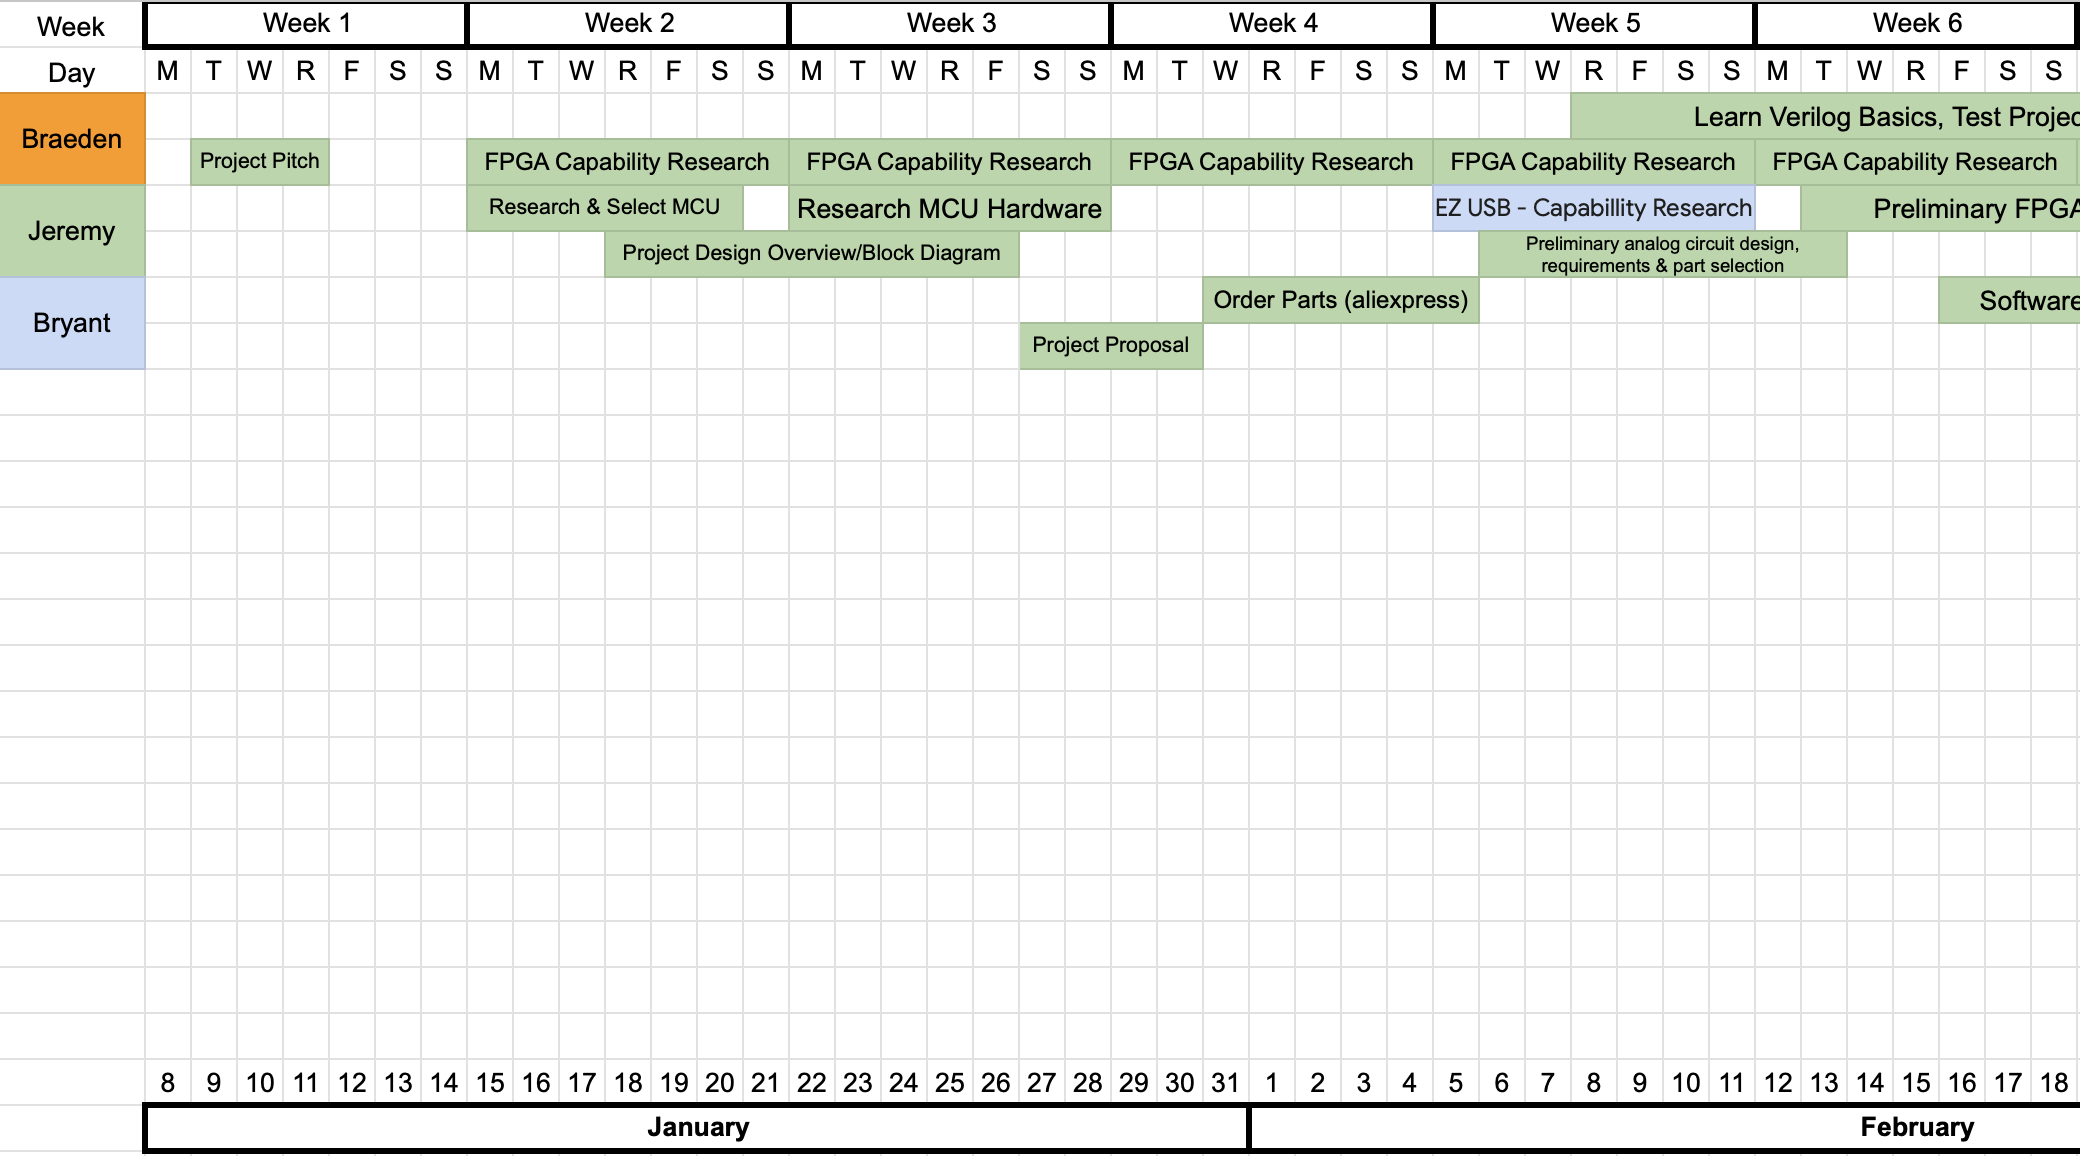
\includegraphics[width=0.8\linewidth]{images/GANTT1.png}
				\caption{GANTT Winter Weeks 1-6}
				\label{fig:gantt1}
				\vspace{15px}
			\end{figure}
			\begin{figure}[H]
				\centering
				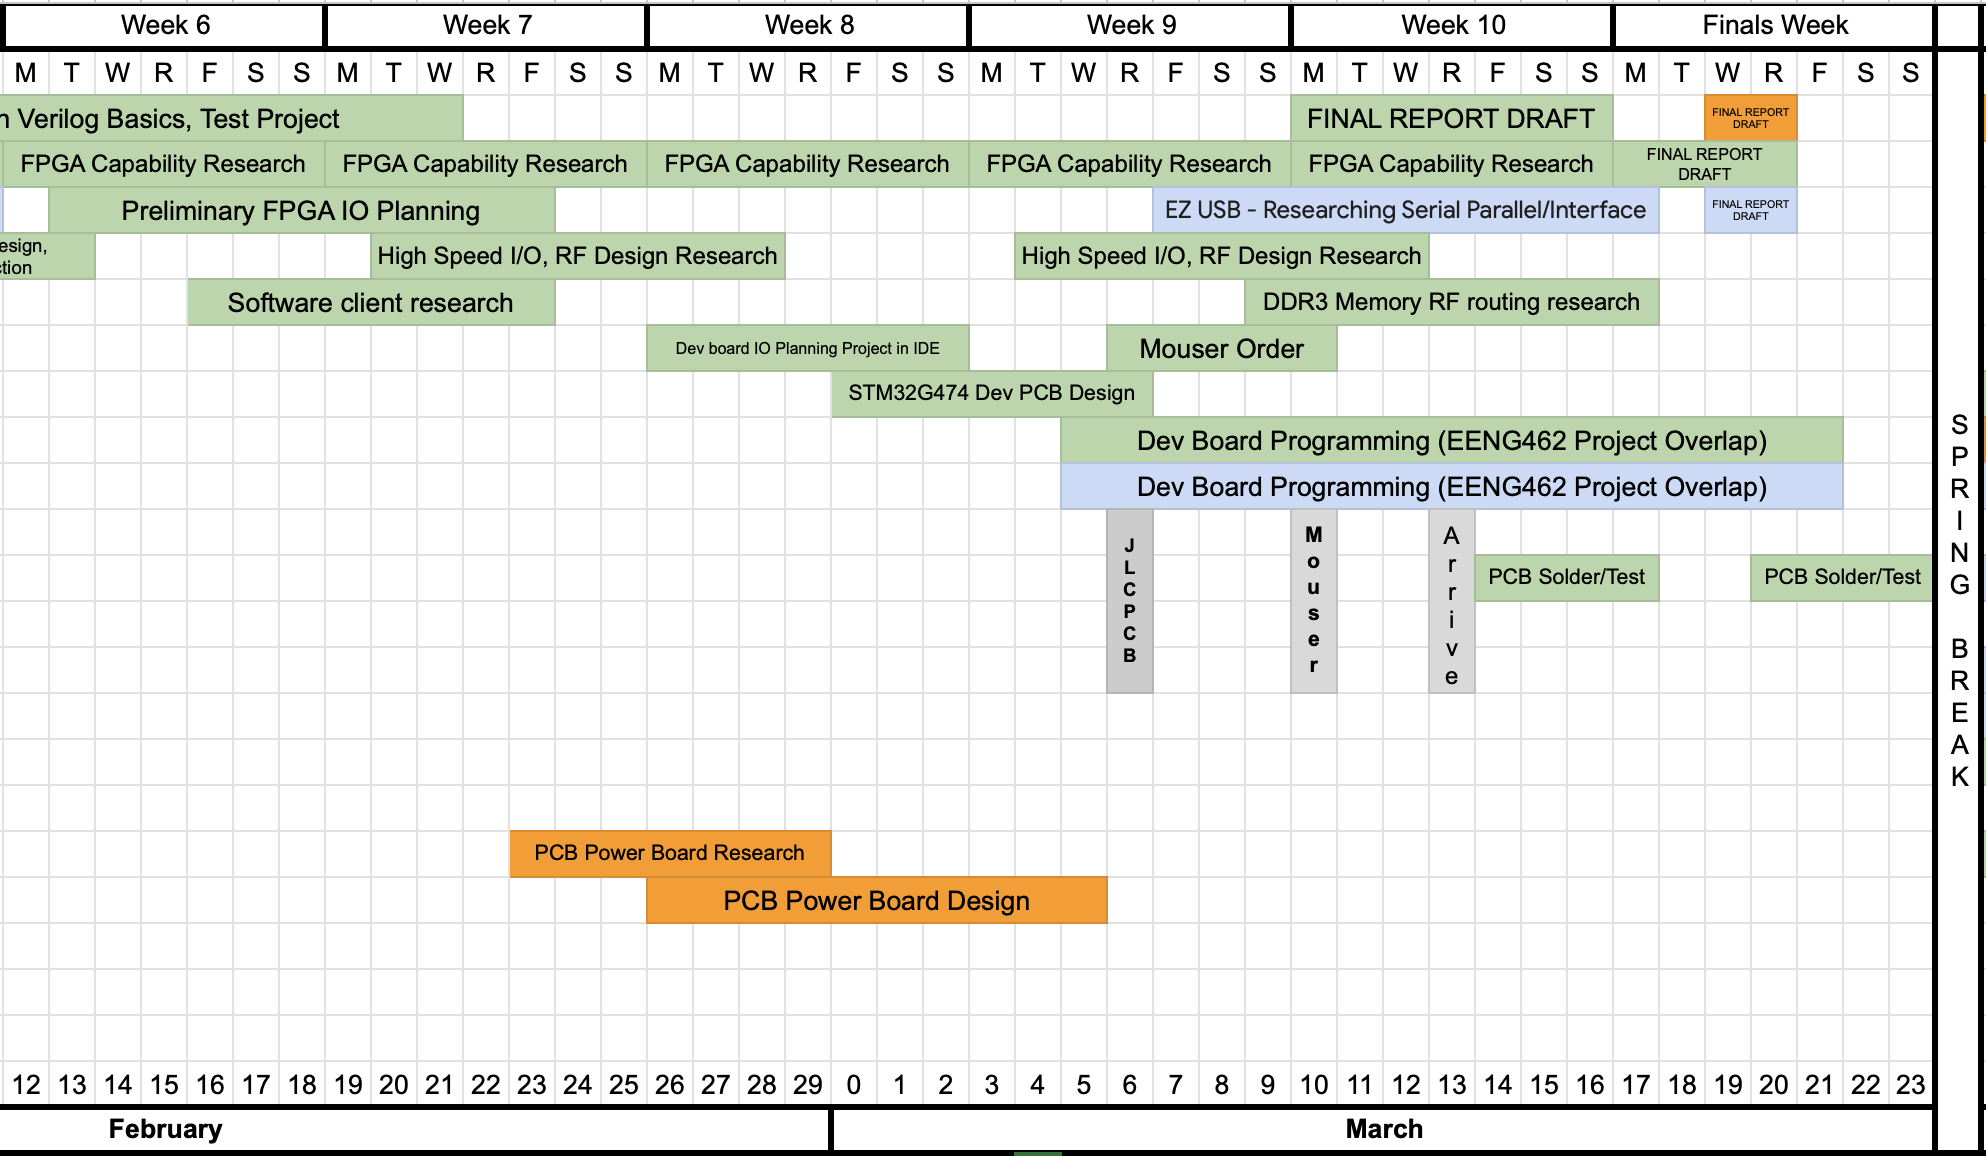
\includegraphics[width=0.8\linewidth]{images/GANTT2.png}
				\caption{GANTT Winter Weeks 6-11}
				\label{fig:gantt2t}
				\vspace{15px}
			\end{figure}
			\begin{figure}[H]
				\centering
				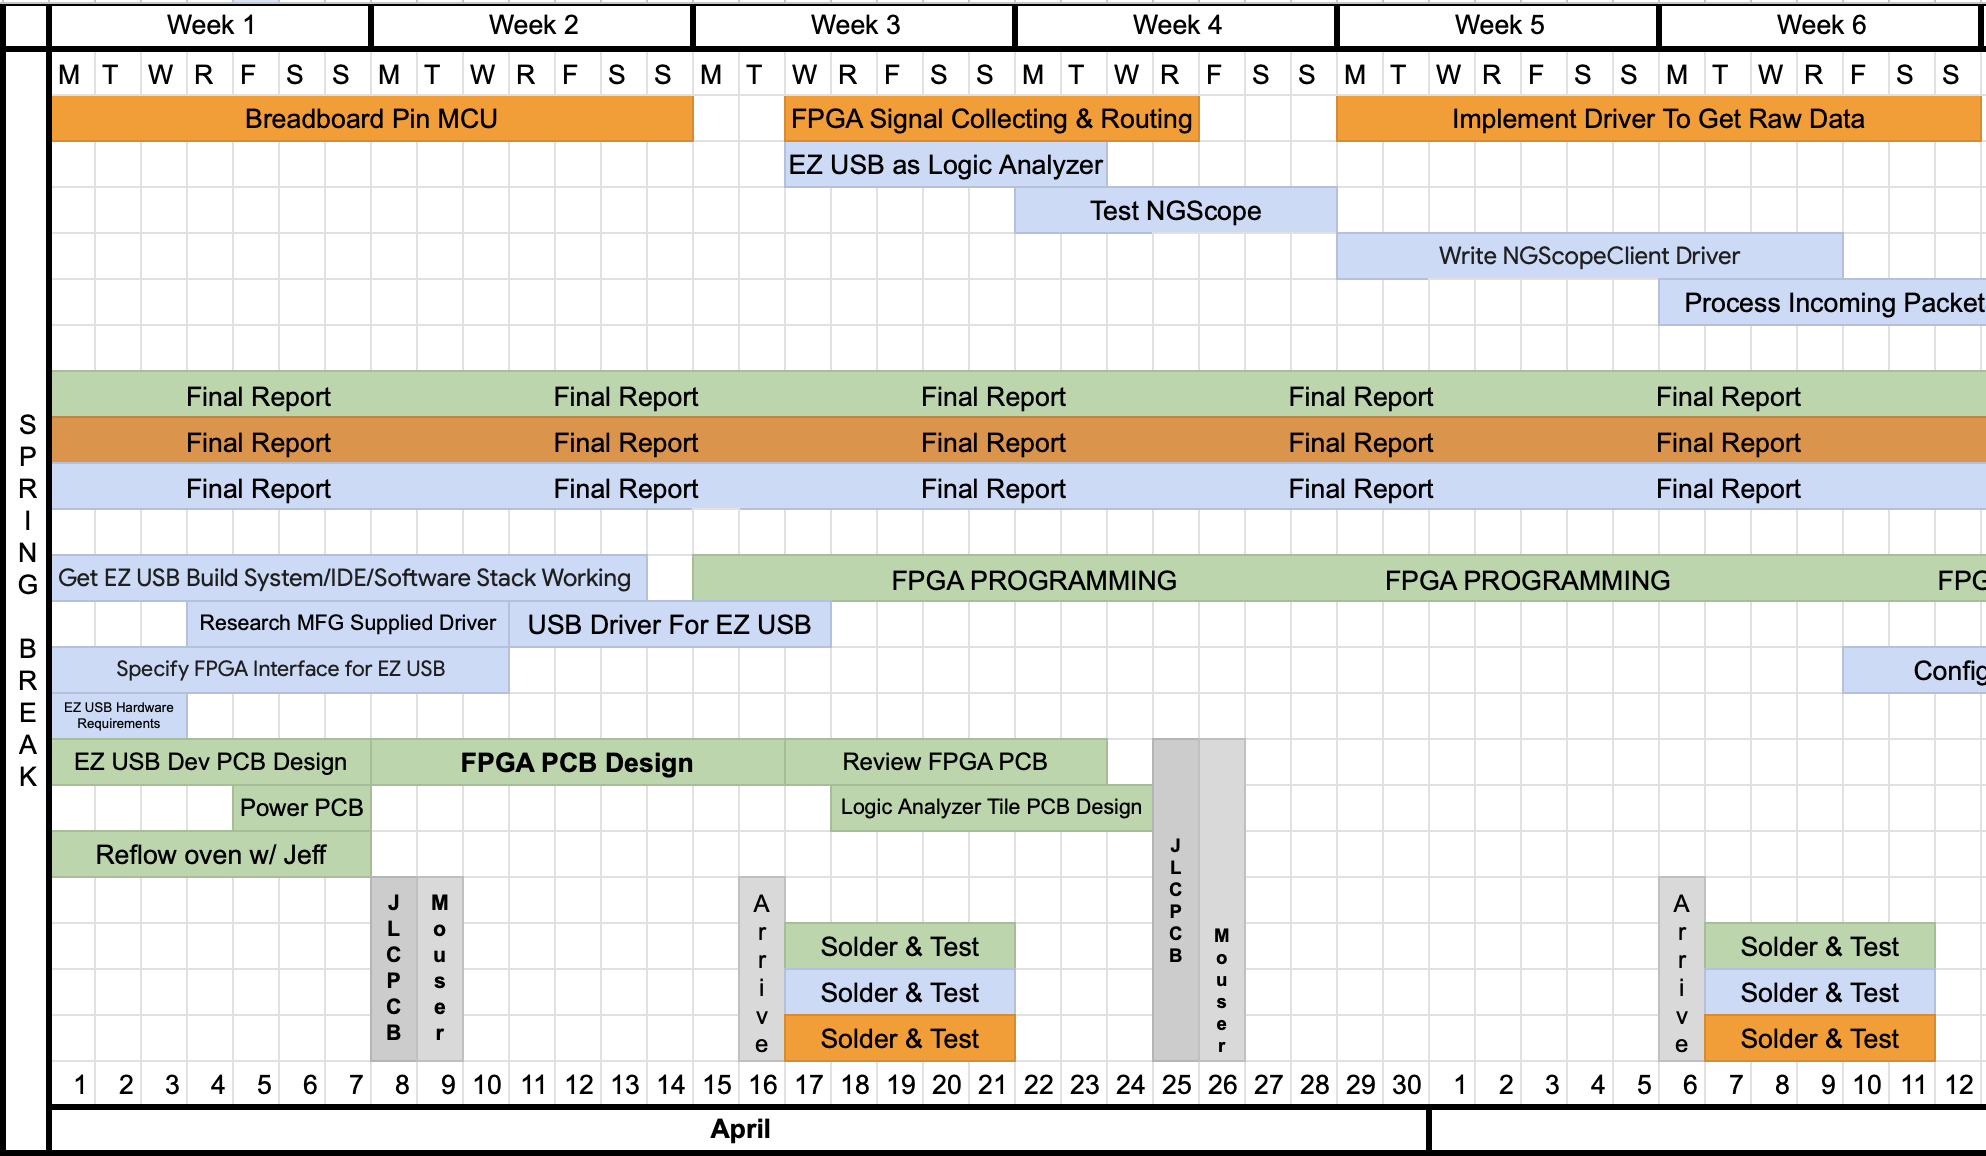
\includegraphics[width=0.8\linewidth]{images/GANTT3.png}
				\caption{GANTT Spring Weeks 1-6}
				\label{fig:gantt3}
				\vspace{15px}
			\end{figure}
			\begin{figure}[H]
				\centering
				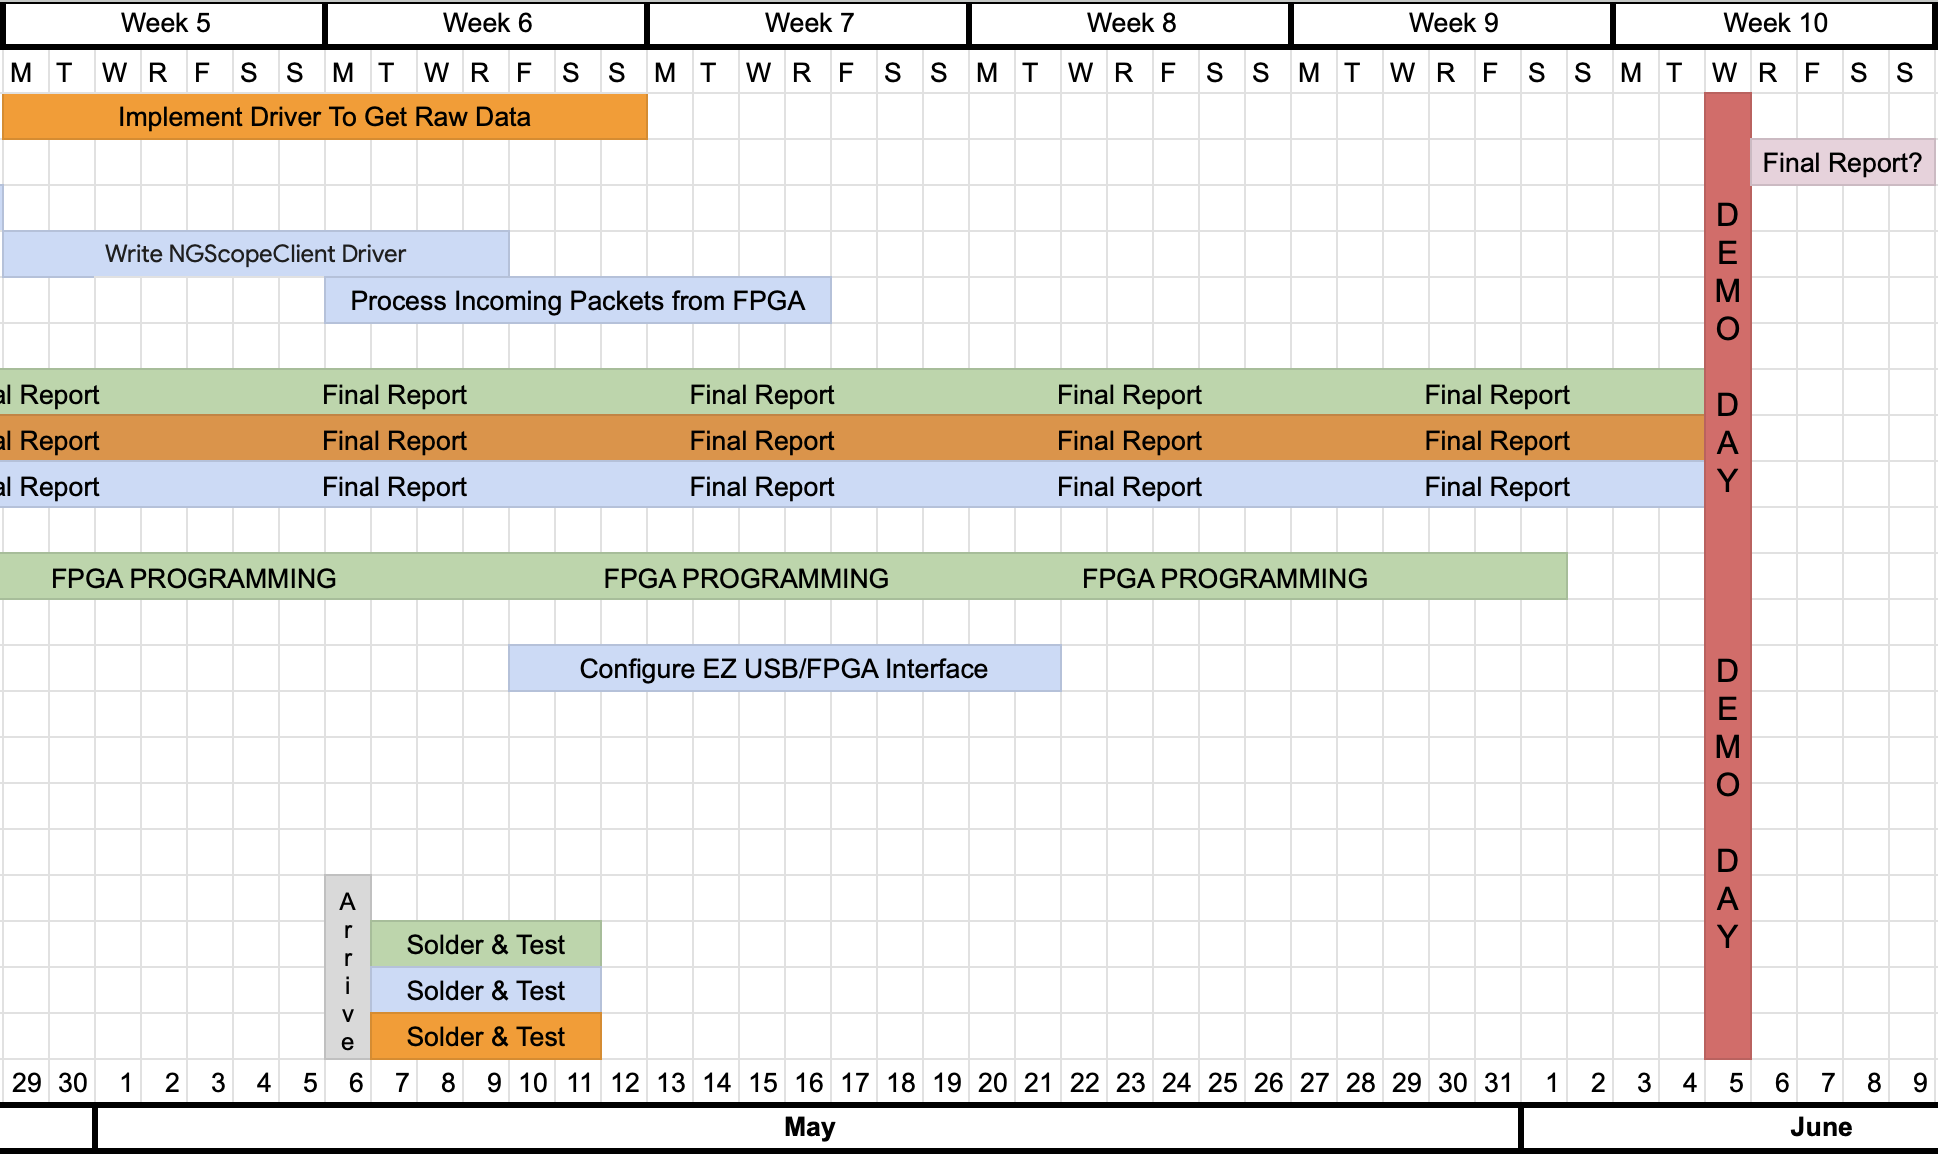
\includegraphics[width=0.8\linewidth]{images/GANTT4.png}
				\caption{GANTT Spring Weeks 5-10}
				\label{fig:gantt4}
				\vspace{15px}
			\end{figure}
			